\section{Mallin testaus}
Keskusyksiköllä laskenta on verrattain hidasta ja esimerkiksi 144 säteellä laskenta kestää noin viisi minuuttia. Tästä syystä SPECT-rekonstruktion validoinnissa käytettiin mallia 3, jolla rekonstruktio onnistuu jo 4 säteellä. Esimerkiksi mallilla 2 onnistunut rekonstruktio vaatii 7 sädettä ja mallissa 1 säteiden minimimäärä on detektorin pikselin päälle asettuvien kollimaattorin reikien lukumäärä, eli useita kymmeniä. Mallia 3 testattiin suorittamalla NEMA-fantomin simuloidun projektiodatan rekonstruktio 100 kertaa. Rekonstruktiossa käytettiin OSEM-algoritmia kahdella iteraatiolla ja 8 osajoukolla. Kuva-alueen koko oli $128^3$ vokselia ja detektorin parametrit kuten simulaatiossa. Laskennassa käytetty suoritin oli Intel i7-10850H.

\begin{figure}[H]
    \centering
    \captionsetup{width=.9\linewidth}
    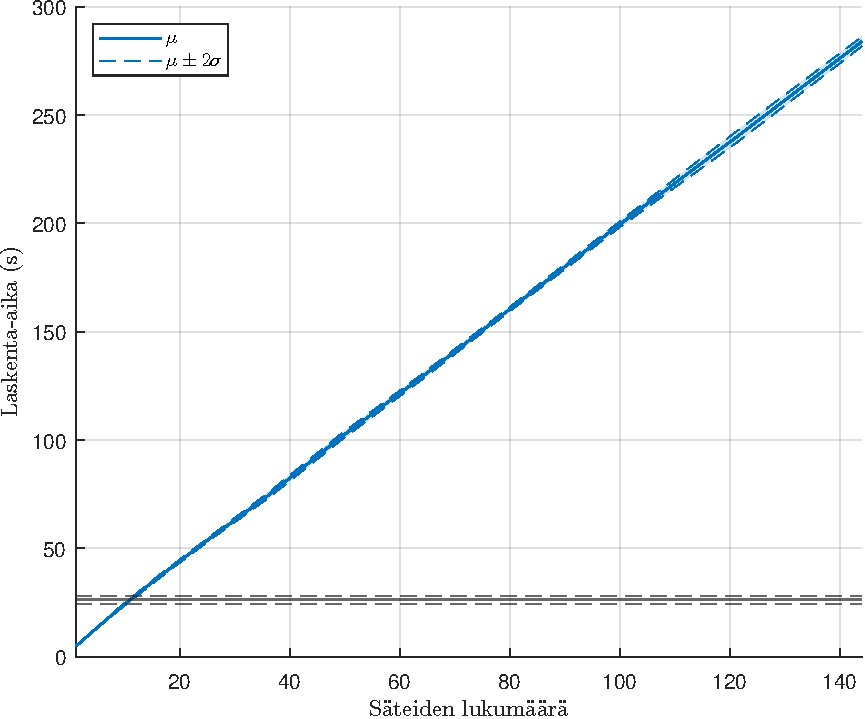
\includegraphics[width=.9\linewidth]{kuvat/laskenta_aika.pdf}
    \caption{Sinisellä viivalla on piirretty mallin 3 keskimääräinen laskenta-aika ($N=100$) säteiden lukumäärän funktiona. Punaisilla katkoviivoilla on havainnollistettu kahden keskihajonnan vaihteluväliä. Rekonstruktiossa kuvan koko oli $128^3$ vokselia sekä algoritmi oli OSEM kahdella iteraatiolla ja 8 osajoukolla. Projektioiden lukumäärä oli 64 ja jokaisessa projektiokuvassa oli $128^2$ pikseliä. Laskennassa käytetty suoritin oli Intel i7-10850H.}
    \label{fig:laskenta_aika}
\end{figure}

\hyperref[fig:laskenta_aika]{Kuvassa \ref*{fig:laskenta_aika}} on esitetty mallin 3 sadan rekonstruktion keskimääräinen laskenta-aika säteiden lukumäärän funktiona sekä kahden keskihajonnan väli. Kuvaajasta nähdään, että käytetyllä laitteistolla laskenta-aika sekunneissa on säteiden lukumäärä kaksinkertaisena. Poikkeuksena on yhdellä säteellä laskettu rekonstruktio, jonka laskenta-aika on selvästi pienempi. Tämä johtuu kuitenkin siitä, että iteratiivisen rekonstruktion arvio kuvasta ei suppene yhdellä säteellä, jolloin laskentaan ei kulu lähes yhtään aikaa. \hyperref[fig:laskenta_aika]{Kuvan \ref*{fig:laskenta_aika}} suoran kulmakerroin riippuu lähinnä laskennassa käytetyn suorittimen tehokkuudesta, iteraatioiden ja osajoukkojen lukumäärästä sekä kuva-alueen ja detektoripaneelin resoluutiosta.

Kuviin \ref{fig:rekonstruktio4}, \ref{fig:rekonstruktio64} ja \ref{fig:rekonstruktio144} on piirretty projektiodatan rekonstruktio 4, 64 ja 144 säteellä. Jokainen rekonstruktioista on selkeä, mutta yksityiskohdat ja muutokset aktiivisuusjakaumassa tarkentuvat säteiden määrän kasvaessa.
\begin{figure}[H]
    \centering
    \captionsetup{width=.9\linewidth}
    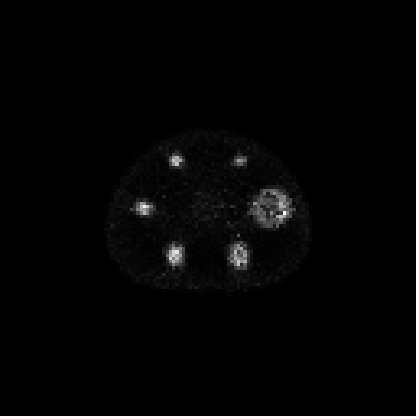
\includegraphics[width=.9\linewidth]{kuvat/rekonstruktio_nRay4.pdf}
    \caption{Projektiodatan rekonstruktio. Mallissa jokainen detektorin pikseli havaitsee gammafotoneja 4 eri suunnasta.}
    \label{fig:rekonstruktio4}
\end{figure}
\begin{figure}[H]
    \centering
    \captionsetup{width=.9\linewidth}
    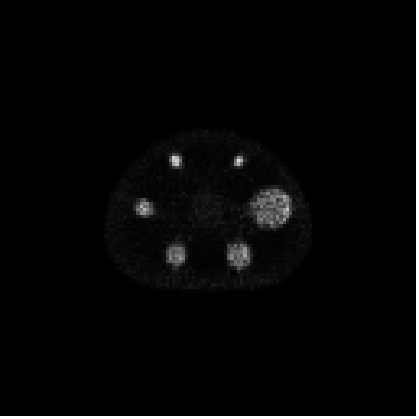
\includegraphics[width=.9\linewidth]{kuvat/rekonstruktio_nRay64.pdf}
    \caption{Projektiodatan rekonstruktio. Mallissa jokainen detektorin pikseli havaitsee gammafotoneja 64 eri suunnasta.}
    \label{fig:rekonstruktio64}
\end{figure}
\begin{figure}[H]
    \centering
    \captionsetup{width=.9\linewidth}
    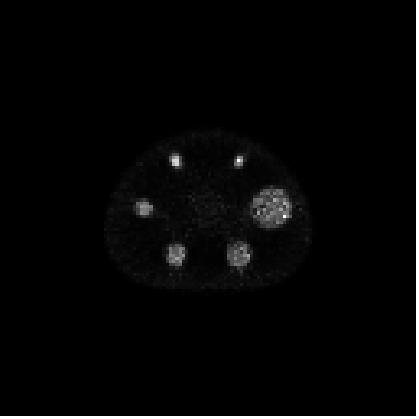
\includegraphics[width=.9\linewidth]{kuvat/rekonstruktio_nRay144.pdf}
    \caption{Projektiodatan rekonstruktio. Mallissa jokainen detektorin pikseli havaitsee gammafotoneja 144 eri suunnasta.}
    \label{fig:rekonstruktio144}
\end{figure}